\documentclass[10pt,twocolumn,journal]{IEEEtran}
% XeLaTeX: all fonts are resolved from the local installation.
\usepackage{fontspec}
\defaultfontfeatures{Ligatures=TeX}
\setmainfont[
  BoldFont=TeXGyreTermes-Bold,
  ItalicFont=TeXGyreTermes-Italic,
  BoldItalicFont=TeXGyreTermes-BoldItalic,
  SmallCapsFont=TeXGyreTermes-Regular,
  SmallCapsFeatures={Letters=SmallCaps}
]{TeXGyreTermes-Regular}
\IfFontExistsTF{Arial}{\setsansfont{Arial}}{\setsansfont{Liberation Sans}}
\setmonofont{TeXGyreCursor-Regular}

\usepackage[margin=1in,bottom=1in]{geometry}
\usepackage{amsmath,amssymb}
\usepackage{booktabs,array,multirow}
\usepackage{graphicx}
\usepackage{xurl}
\usepackage{xr-hyper}
\usepackage[hidelinks]{hyperref}
\urlstyle{same}
\usepackage{fancyhdr}
\usepackage{flushend}
\externaldocument{supplement}[supplement.pdf]
\graphicspath{{figures/}}
\setlength{\emergencystretch}{4em}
\pagestyle{fancy}
\fancyhf{}
\fancyhead[L]{\scriptsize BELOW ZERO}
\fancyhead[R]{\scriptsize\thepage}
\renewcommand{\headrulewidth}{0pt}
\hypersetup{pdftitle={Below Zero: Spatially Adaptive Conditional Readout Sampling for Lower-Censored RAW Images},pdfauthor={},pdfsubject={Spatially adaptive conditional sampling of lower-censored RAW readouts}}
\newcommand{\BZAuthorBlockEN}{Yaogeng Jiang\\Independent Researcher\\\href{mailto:y.g.jiang@sjtu.edu.cn}{y.g.jiang@sjtu.edu.cn}}
\newcommand{\BZAuthorBlockZH}{姜尧耕\\独立研究者\\\href{mailto:y.g.jiang@sjtu.edu.cn}{y.g.jiang@sjtu.edu.cn}}
\newcommand{\BZPDFAuthors}{Yaogeng Jiang}

\hypersetup{pdfauthor={\BZPDFAuthors}}
\begin{document}
\title{{\normalsize \href{https://github.com/y-g-jiang/Video-RAW-Black-Level-Correction-Net/tree/main/below_zero}{Code and data}}\\[6pt]Below Zero: Spatially Adaptive\\Conditional Readout Sampling\\for Lower-Censored RAW Images}
\author{\BZAuthorBlockEN}
\maketitle
\thispagestyle{fancy}

\begin{abstract}
Clipping black-level-subtracted RAW sensor measurements at zero discards negative readout codes and distorts shadow statistics. We present a single-frame completion method, N0/PG, that samples signed integers at lower-censored locations while preserving every positive measurement. A multiscale convolutional estimator predicts the local optical signal, and a calibrated quantized Poisson--Gaussian (PG) decoder maps each prediction to the conditional probability distribution over zero and negative integer codes, so re-clipping the completed Bayer frame at zero reproduces the input exactly. Under a calibrated high-gain sensor profile across 138 held-out source images, N0/PG reduces mean excess Kullback--Leibler (KL) divergence from 0.001723 to 0.000313~nats relative to local maximum-likelihood estimation, improving KL on every source image and lowering the negative log-likelihood of withheld integer codes by 0.001407~nats per censored pixel. Stratified analyses show that classical local estimators are already accurate in uniform near-black regions, whereas multiscale context yields large gains at higher signal levels and in structured neighborhoods. Moreover, permuting the predicted distributions across censored locations substantially increases error, confirming that accurate spatial assignment is critical. On two real exposures with retained signed references and on a controlled color-rendering benchmark, conditional readout sampling recovers demosaicked shadow variation and reduces clipping-induced color bias. These results establish a measurement-preserving framework for lower-censored RAW completion and quantify the contribution of learned spatial estimation to conditional readout accuracy.
\end{abstract}

\begin{IEEEkeywords}
Computational imaging, censored measurements, Bayer raw images, Poisson--Gaussian noise, probabilistic reconstruction, demosaicking.
\end{IEEEkeywords}

\section{Introduction and Related Work}
In RAW sensor pipelines, subtracting the nominal black level centers measurements around a signed origin. Even when the optical signal is nonnegative, electronic read noise produces negative codes in dark regions. Truncating these codes to zero alters the mean and variance of the observed noise \cite{foi2008,foi2009} and biases subsequent averaging and interpolation. Such lower clipping appears in documented camera pipelines \cite{mathworksISP}, raw-file investigations \cite{librawD5300,claffReadNoise}, and the clipped negative noise analyzed by the VMCL-ISP team in the AIM 2025 low-light RAW video challenge \cite{aim2025Video}, while standard RAW evaluation interfaces likewise enforce nonnegative output constraints \cite{sonyAIM2025}.

Our goal is to complete a single lower-censored Bayer frame with statistically plausible signed integer readouts. Zero clipping merges the native quantized zero code and all negative integer codes into a single observation $Y_i=0$. Completion must sample missing nonpositive codes at censored pixels while leaving all positive measurements intact, thereby preserving the sensor measurement representation for downstream stages.

The key difficulty is that identical observed zeros need not share the same conditional readout law. A zero adjacent to an illuminated edge carries different evidence about the hidden readout than a zero inside a uniform shadow. Nearby positive measurements encode this structural difference, whereas locally constant signal models tend to smooth it away. Once a spatially varying signal field is estimated from surrounding context, a single calibrated decoder can assign distinct readout distributions across structural regimes.

To this end, N0/PG decouples spatial signal estimation from physical conditional decoding (Fig.~\ref{fig:pipeline}). A NAF-style convolutional network \cite{nafnet} predicts a nonnegative signal field from packed Bayer observations and calibration constants, and a calibrated quantized Poisson--Gaussian (PG) decoder evaluates the conditional distribution over zero and negative integers given $Y_i=0$. The sampler fills only censored pixels, while an identity branch copies every positive code verbatim.

\begin{figure*}[t]
\centering
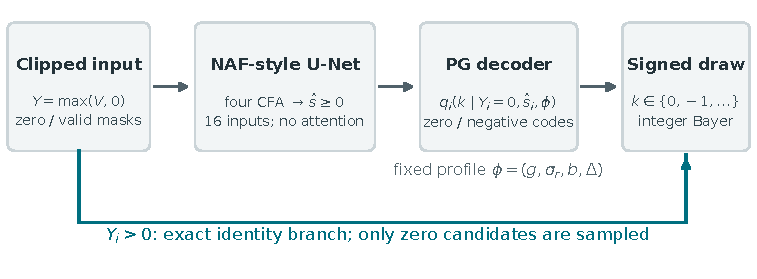
\includegraphics[width=\textwidth]{f01_pipeline.pdf}
\caption{Spatially adaptive signed-RAW completion. The network predicts local signal parameters for the quantized PG decoder. Censored pixels ($Y_i=0$) are sampled from the resulting conditional distribution over nonpositive integers, while observed positive codes ($Y_i>0$) pass through the identity branch unchanged.}
\label{fig:pipeline}
\end{figure*}

We examine whether learned spatial context estimates conditional readout laws more accurately than local noise-model fitting and transform-domain filtering. We evaluate distributional accuracy across 138 held-out source images, analyze how gains depend on signal level and neighborhood structure, and test how completed signed samples affect demosaicking and fixed color rendering.

\subsection{Related Work}
\subsubsection{Censored Measurements and RAW Noise Models}
Conditional imputation is a standard approach to censored observations. In Tobit regression, O'Neill \cite{oneill2024} uses latent-data augmentation to retain uncensored responses while drawing censored outcomes from their conditional laws. In computational imaging, Kodgirwar et al.\ \cite{kodgirwar2024} infer saturated Poisson counts for multi-exposure ptychographic fusion. Here we formulate single-frame Bayer readout completion under quantized PG noise, preserving both observed positive codes and the discrete probability mass of a native zero readout.

Foi et al.\ \cite{foi2008} established practical PG noise modeling with clipping for RAW data, and Foi \cite{foi2009} derived forward transforms and inverse bias corrections for denoising clipped heteroskedastic observations. Our conditional decoder builds on this statistical model, but whereas denoising estimates the underlying clean signal, our output is a sampled integer readout at each censored pixel. Our Foi-qPG baseline applies Foi's clipped-noise transforms and collaborative filtering prior to the same quantized conditional decoder used by the other estimators (Section~\ref{sec:baselines}).

Physical RAW sensors also exhibit effects beyond independent Gaussian read noise. Wei et al.\ \cite{wei2020} model low-light sensor noise components, Zhang et al.\ \cite{zhang2021} address correlated noise and quantization, and Mohammadi et al.\ \cite{mohammadi2026} study black-level bias. Even when positive codes are unchanged, such effects can alter the conditional distribution of discarded negative codes.

\subsubsection{Learned Estimation and Conditional Sampling}
NAFNet \cite{nafnet} provides efficient convolutional blocks for image restoration. We use a self-contained NAF-style encoder--decoder without pooled channel attention so that each prediction has a bounded spatial receptive field. Its output is a nonnegative signal parameter in DN, while the calibrated PG model determines the corresponding probabilities.

Combining learned priors with measurement models is central to deep equilibrium reconstruction \cite{gilton2021}, neural convex regularizers \cite{goujon2023}, and Bayesian inversion with generative priors \cite{bohra2022}. Whereas those methods infer a latent clean image, our unknown is the discarded integer readout given $Y_i=0$. Motivated by the analysis of non-blind Poisson deconvolution by Gnanasambandam et al.\ \cite{gnanasambandam2024}, we isolate the effect of spatial estimation and evaluate the resulting conditional distributions with strictly proper scoring rules \cite{gneiting2007}.

\subsubsection{Demosaicking and Downstream Processing}
Joint demosaicking and denoising methods exploit spatial and cross-channel correlations to recover clean RGB images \cite{gharbi2016}. Our task operates earlier in the pipeline by completing plausible signed measurements prior to interpolation, which we test using adaptive homogeneity-directed (AHD) demosaicking \cite{hirakawa2005} in a pinned LibRaw implementation \cite{libraw}.

\section{Conditional Readout Completion}
\subsection{Quantized Lower-Censored Readouts}
Let $s_i\geq0$ denote the expected optical signal in DN, $g$ the conversion gain in DN/e$^{-}$, and $b_i$ a known offset relative to the nominal black level. Under the calibrated PG model, the photon count $N_i$ and continuous signed readout $Z_i$ satisfy
\begin{align}
N_i&\sim\operatorname{Poisson}(s_i/g),\label{eq:pois}\\
Z_i&=gN_i+b_i+\epsilon_i,\qquad \epsilon_i\sim\mathcal N(0,\sigma_r^2).\label{eq:forward}
\end{align}
Rounding to the nearest integer with a 1-DN step gives $V_i=\lfloor Z_i+1/2\rfloor$. Choosing a common signed origin places the clipping floor at zero (floors at other file-domain codes are represented by shifting this origin). Lower censoring then yields
\begin{equation}
Y_i=\max(V_i,0),\qquad \mathcal Z=\{i:Y_i=0\}.\label{eq:censor}
\end{equation}
The simulator includes upper saturation at $16383-512=15871$~DN. Evaluated realizations remain above the physical lower bound of the ADC, where we model readout noise as an unbounded Gaussian.

For $k\leq0$, the unconditional probability mass of quantized code $k$ is
\begin{align}
a_k(s,b)=\sum_{n=0}^{\infty}\operatorname{Pois}(n;s/g)
\bigg[&\Phi\!\left(\frac{k+1/2-gn-b}{\sigma_r}\right)\nonumber\\[-2pt]
-&\Phi\!\left(\frac{k-1/2-gn-b}{\sigma_r}\right)\bigg],\label{eq:bin}
\end{align}
where $\Phi$ is the standard normal cumulative distribution function. The zero-observation probability is
\begin{equation}
c(s,b)=\sum_{n=0}^{\infty}\operatorname{Pois}(n;s/g)
\Phi\!\left(\frac{1/2-gn-b}{\sigma_r}\right).\label{eq:zeroevent}
\end{equation}
The $+1/2$~DN upper boundary encompasses both the quantization bin of the native zero code and all negative integer bins.

Given a signal estimate $\hat s_i$, the decoder returns
\begin{equation}
q_i(k)=\frac{a_k(\hat s_i,b_i)}{c(\hat s_i,b_i)},\qquad k=0,-1,-2,\ldots.\label{eq:posterior}
\end{equation}
Bin integration in \eqref{eq:bin} preserves the discrete atom at $k=0$, while normalization in \eqref{eq:posterior} conditions on the complete zero-observation event. Fig.~\ref{fig:counterexamples} shows how the resulting distribution varies across image locations.

\subsection{Measurement-Preserving Completion}
At each zero candidate $i\in\mathcal Z$, we draw $K_i$ from its predicted conditional law $q_i$ and construct
\begin{equation}
\widetilde V_i=\begin{cases}
Y_i,&Y_i>0,\\
K_i,\quad K_i\sim q_i,&Y_i=0.
\end{cases}\label{eq:output}
\end{equation}
The identity branch and the nonpositive support of $q_i$ guarantee $\max(\widetilde V_i,0)=Y_i$ exactly. A conditional sample expresses the hidden readout fluctuation rather than a point estimate of the clean signal, so random sampling and conditional means optimize different losses. We evaluate $q_i$ with proper distribution scores, and derive the risk identities comparing sampling with conditional means in Supplementary Section~I.

Using the true $s_i$, the simulator defines the known-signal reference law
\begin{equation}
p^{\star}_i(k)=a_k(s_i,b_i)/c(s_i,b_i)\label{eq:oracle}
\end{equation}
at each censored pixel. At inference time, fixing the estimated signal field $\hat s_i$ makes $q_i$ a plug-in conditional readout law, and samples are drawn independently across pixels given $\hat s$.

\section{Learning Spatially Adaptive Readout Laws}
\subsection{Signal Estimator}
We pack the Bayer phases as $[R,G_1,G_2,B]$ and supply transformed measurements, zero-candidate indicators, known offsets, a validity mask, and calibration constants. The validity mask distinguishes padded border pixels from measured zeros, while the offsets enter both the estimator and the PG decoder.

Our four-stage NAF-style encoder--decoder fuses multiscale features through additive skip connections and pixel-shuffle upsampling. Pointwise channel normalization, depthwise convolutions, and multiplicative SimpleGates provide a bounded spatial receptive field without global pooling or attention. A four-channel softplus head predicts $\hat s_i\geq0$ in DN, which the decoder converts to photoelectron means $\hat s_i/g$. The model has 10,913,380 parameters, with channel definitions and stage dimensions listed in Supplementary Section~II.

\subsection{Training With a Conditional-Distribution Target}
In synthetic training, the ground-truth signal $s_i$ defines the conditional target $p_i^\star$, and we minimize the average cross-entropy over valid zero candidates:
\begin{equation}
\mathcal L(\theta)=-\frac{1}{|\mathcal Z|}
\sum_{i\in\mathcal Z}\sum_{k\leq0}p^{\star}_i(k)\log q_{\theta,i}(k).
\label{eq:loss}
\end{equation}
We evaluate \eqref{eq:loss} on a finite categorical representation with an explicit tail bin. Because the target entropy $H(p_i^\star)$ is independent of $\theta$, minimizing \eqref{eq:loss} minimizes the KL divergence from $p_i^\star$ to $q_{\theta,i}$. Gradients pass through the physical decoder to the estimator so that signal predictions are optimized directly for conditional distribution accuracy. Because the decoder receives known calibration constants and per-realization offsets, optimization updates only the spatial estimator.

\subsection{Discrete Support and Coordinate-Indexed Sampling}
The categorical distribution explicitly represents codes $0,-1,\ldots,-304$ and groups $V\leq-305$ into a single tail bin. When evaluating likelihoods or sampling within this tail bin, the conditional PG law is resolved to individual integer codes. Supplementary Section~III details tail evaluation, numerical error bounds, and order-invariant coordinate-indexed sampling.

\begin{figure*}[t]
\centering
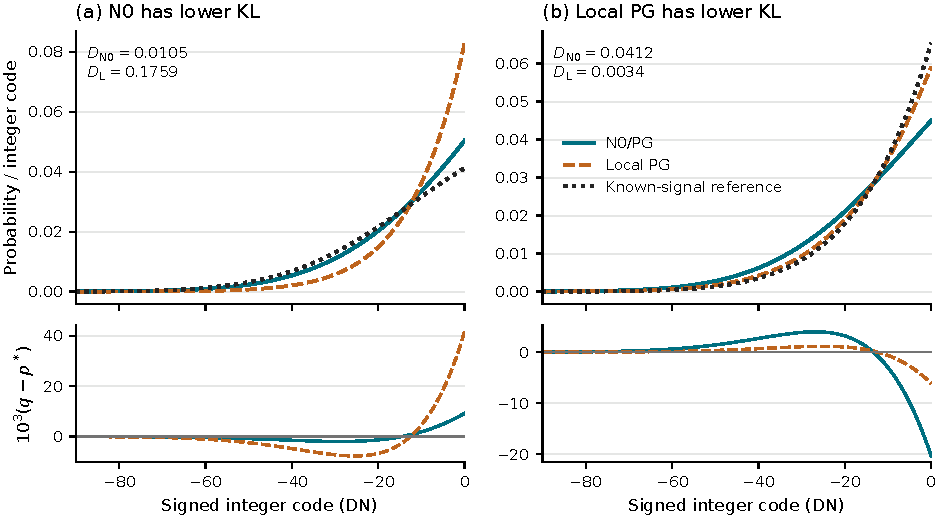
\includegraphics[width=\textwidth]{f02_pmf_counterexamples.pdf}
\caption{Conditional PMFs at two high-gradient development locations, selected after evaluation to illustrate cases where each estimator is more accurate. The top row shows N0/PG, Local PG, and the known-signal law, and the bottom row shows signed probability error. N0 is more accurate in (a), whereas Local PG is more accurate in (b).}
\label{fig:counterexamples}
\end{figure*}

\section{Experiments}
\subsection{Data, Calibration, and Training}
Experiments use the calibrated Panasonic S5~II ISO12800 parameters in Table~\ref{tab:protocol}. Gain $g$ comes from JOT measurements \cite{jot}, and read noise is estimated from ten dark frames using the R and $G_1$ phases. Because the synthetic generator, reference laws, and conditional decoder share this PG model, the held-out test isolates spatial conditional-law estimation under matched noise assumptions, while retained real readouts test the same model on camera data.

\begin{table}[t]
\centering
\caption{Calibrated sensor parameters and experimental settings.}
\label{tab:protocol}
\small
\begin{tabular}{@{}p{0.40\columnwidth}p{0.52\columnwidth}@{}}
\toprule
Item & Setting\\
\midrule
Sensor setting & S5 II, ISO12800, mechanical shutter, 14 bit\\
Gain $g$ & 21.6010924121 DN/e$^{-}$\\
Integer read-noise RMS & 24.9612744275 DN\\
Analog $\sigma_r$ & 24.9596051193 DN\\
Nominal black level / step & 512 DN / 1 DN\\
Synthetic offset $b_c$ & Known, uniform $[-0.25,0.25]$ DN\\
Source-image split & 825 train / 137 dev / 138 test\\
Training & Seed 7103, 80,000 updates\\
Test contexts / target core & 128 and 256 / central 64 packed pixels\\
\bottomrule
\end{tabular}
\end{table}

Synthetic signal fields use 1,100 color templates from DIV2K and BSDS500 \cite{div2k,bsds500}, split into 825 training, 137 development, and 138 test sources. Training draws comprise 90\% natural scenes and 10\% procedural controls, with exposure, color variation, quantization, and censoring generated as in Supplementary Section~II. A single trained N0 checkpoint is selected using the development set.

Each held-out source generates two scenes with independent exposures and noise seeds, evaluated under nested 128- and 256-pixel contexts sharing a central 64-pixel target. Across the 138 sources, this yields 552 cases and 3,254,612 scored candidates (1,627,306 unique candidate locations in the 256-pixel context).

\subsection{Baseline Estimators}\label{sec:baselines}
Global PMF uses the empirical average conditional distribution from the training data for each CFA phase, while Global PG plugs the training-fitted phase signal into the calibrated decoder, so both produce spatially constant predictions at test time.

Local PG fits a signal by maximum likelihood in a same-CFA $5\times5$ neighborhood using positive codes and zero-censoring events. Local Bayes combines this likelihood with a fitted zero-plus-Gamma signal prior and integrates the resulting conditional laws. Both use the development-selected $5\times5$ window and count the center event once.

Foi-qPG applies Foi's clipped-noise transform \cite{foi2009} and BM3D filtering \cite{bm3d}, followed by quantized PG inversion and the shared conditional integer decoder.

Whereas N0 uses all four CFA phases across multiple scales, the primary local baselines use only same-CFA observations. Our development-set Joint-CFA Bayes control also observes all four phases within a $5\times5$ window to test whether local cross-phase pooling closes the error gap (Supplementary Section~VII-A).

\subsection{Evaluation Criteria}
For each withheld signed integer code $v_i$, we evaluate the predicted conditional distribution $q_i$ with negative log-likelihood (NLL) and the discrete continuous ranked probability score (CRPS):
\begin{align}
\mathrm{NLL}(q_i,v_i)&=-\log q_i(v_i),\label{eq:nll}\\
\mathrm{CRPS}(q_i,v_i)&=\sum_{k\in\mathbb Z}
\left(F_{q_i}(k)-\mathbf{1}\{v_i\leq k\}\right)^2\Delta.\label{eq:crps}
\end{align}
NLL is in nats per candidate and CRPS is in DN with $\Delta=1$~DN, and both evaluate the exact withheld integer code by resolving individual codes within the tail bin.

When the simulated signal $s_i$ is known, we also compare $q_i$ directly with the true conditional law $p_i^\star$ via excess KL divergence and cumulative distribution discrepancy:
\begin{align}
D_i&=\sum_{k\leq0}p^{\star}_i(k)\log\frac{p^{\star}_i(k)}{q_i(k)},\label{eq:kl}\\
J_i&=\sum_{k\in\mathbb Z}\left(F_{q_i}(k)-F_{p^{\star}_i}(k)\right)^2\Delta.\label{eq:cdf}
\end{align}
Excess KL and $J_{\mathrm{CDF}}$ use the shared 306-category support with an aggregated tail bin, whereas NLL and CRPS resolve individual tail integers (Supplementary Section~III).

Scores are aggregated within each source image and then averaged across sources with equal weight. Paired source bootstrap resampling keeps all related cases of a source together. The two primary KL comparisons against Local Bayes and Foi-qPG use 97.5\% intervals, while secondary comparisons use 95\% intervals (Supplementary Sections~\ref{sec:scoreaggregation} and~\ref{sec:regionaldefinitions}).

\subsection{Conditional-Distribution Accuracy on Held-Out Data}
N0/PG achieves the lowest excess KL, $J_{\mathrm{CDF}}$, NLL, and CRPS among the evaluated methods (Table~\ref{tab:holdout}). The known-signal law establishes the reference level attainable within the simulator, whereas deterministic zero fill cannot assign nonzero probability to negative codes.

\begin{table*}[t]
\centering
\caption{Conditional-distribution scores on 138 held-out source images (four related case/context combinations per source, equal source weighting). Excess KL and $J_{\mathrm{CDF}}$ use the 306-category support, while NLL and CRPS resolve the integer tail. Boldface indicates the best deployable method. Zero fill assigns zero probability to negative labels, yielding infinite KL/NLL, and the known-signal reference uses the true underlying signal.}
\label{tab:holdout}
\small
\begin{tabular}{@{}llrrrr@{}}
\toprule
Method & Available spatial information & $10^3D_{\mathrm{KL}}\downarrow$ & NLL$\downarrow$ & CRPS$\downarrow$ & $10^3J_{\mathrm{CDF}}\downarrow$\\
\midrule
Zero fill & None & $\infty$ & $\infty$ & 18.691235 & 10611.0233\\
Global PMF & Per-CFA training law & 3.4350 & 3.914828 & 8.112251 & 29.6469\\
Global PG & Per-CFA training signal & 3.3399 & 3.914723 & 8.111302 & 28.7879\\
Local PG & Same-CFA $5\times5$ & 1.7228 & 3.912975 & 8.095007 & 13.7075\\
Local Bayes & Same-CFA $5\times5$ & 1.8429 & 3.913102 & 8.096170 & 14.8024\\
Foi-qPG & Same-CFA image plane & 2.1475 & 3.913454 & 8.100521 & 18.5915\\
N0/PG (ours) & Four-CFA multiscale & \textbf{0.3125} & \textbf{3.911568} & \textbf{8.084118} & \textbf{2.6423}\\
Known-signal reference & Unavailable true signal & 0.0000 & 3.911245 & 8.081423 & 0.0000\\
\bottomrule
\end{tabular}
\end{table*}

The primary KL differences for N0 minus Local Bayes and Foi-qPG are $-1.5304\times10^{-3}$ and $-1.8350\times10^{-3}$~nats, with 97.5\% intervals of $[-2.1085,-1.0776]\times10^{-3}$ and $[-2.1474,-1.5372]\times10^{-3}$. Relative to Local PG, excess KL drops from $1.722793\times10^{-3}$ to $3.125067\times10^{-4}$~nats, an 81.86\% reduction.

Relative to Local PG, NLL decreases by 0.001407~nats per candidate (95\% interval $[-0.001950,-0.000969]$) and CRPS decreases by 0.010890~DN (interval $[-0.014860,-0.007683]$). The relative reduction in excess KL greatly exceeds that in total NLL because expected log-loss includes conditional readout entropy that no signal estimator can remove. Fig.~\ref{fig:holdout} shows both absolute scores and paired differences.

Across the test set, N0 achieves lower KL on all 138 sources (median reduction 0.0004693~nats), lower NLL on 130 sources, and lower CRPS on 131 sources.

\begin{figure*}[t]
\centering
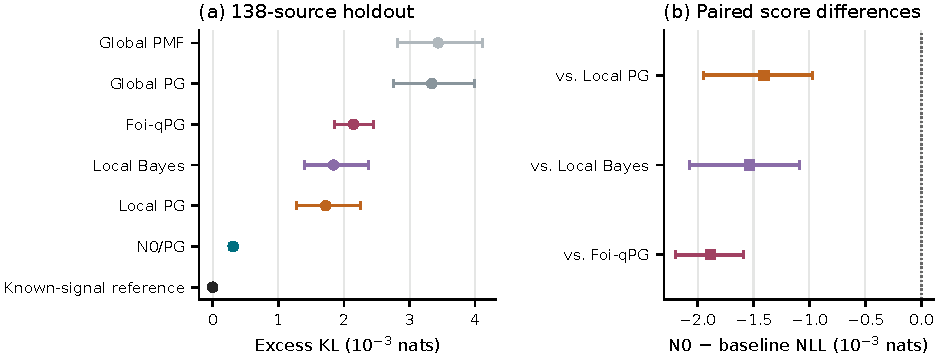
\includegraphics[width=\textwidth]{f03_holdout.pdf}
\caption{Conditional-distribution accuracy on the held-out test set. (a) Mean excess KL and 95\% source-bootstrap intervals. (b) Paired NLL differences relative to N0 with 95\% intervals, where negative values favor N0. The primary 97.5\% comparison intervals are reported in the text.}
\label{fig:holdout}
\end{figure*}

\subsection{Dependence on Signal and Neighborhood Structure}\label{sec:regions}
Because a zero near a bright edge differs from one in a uniform shadow in both its latent signal and its visible neighborhood cues, spatial estimation gains vary across regimes. Fig.~\ref{fig:spatial} stratifies excess KL by signal strength, local variation, edge distance, and observed zero fraction (Supplementary Section~\ref{sec:regionaldefinitions}).

\subsubsection{Signal Level}
Near-black distributions are governed mainly by the calibrated read-noise tail, so different signal estimates yield similar laws. Accordingly, the mean excess-KL difference between N0 and Local Bayes is $-0.000087$~nats for $s<0.25$~DN, but widens to $-0.002887$~nats for $8\leq s<16$~DN. Foi-qPG has lower mean error below 2~DN, whereas N0 is lower above 4~DN (Fig.~\ref{fig:spatial}(a)).

\subsubsection{Neighborhood Variation}
Neighborhood structure strongly modulates the error gap, as N0 minus Local Bayes KL grows from $-0.000358$~nats for $t<0.025$ (379,366 candidates across 115 sources) to $-0.004467$~nats for $t\geq0.8$ (98,229 candidates across 106 sources). Likewise, the difference is $-0.002200$~nats at thresholded gradient locations versus $-0.000330$~nats at distances of at least 16 packed pixels.

From the measurement side, N0 minus Local Bayes KL is $-0.008058$~nats when the observed zero fraction satisfies $z<0.1$ (17,450 candidates), versus $-0.000226$~nats when $0.5\leq z<0.75$ (498,135 candidates), so the gap is largest when a censored pixel is surrounded mostly by positive codes. Because signal strength and local variation are correlated, Section~\ref{sec:gradientcontrol} compares gradient differences matched within source, CFA, and signal bins.

\begin{figure*}[t]
\centering
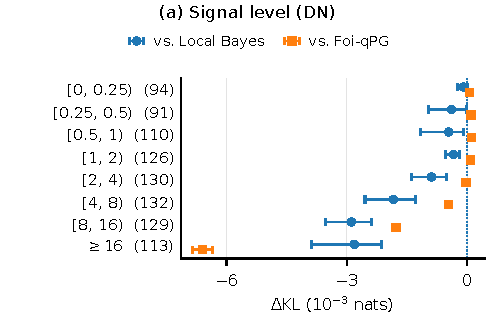
\includegraphics[width=0.493\textwidth]{f10a_holdout_signal.pdf}\hfill
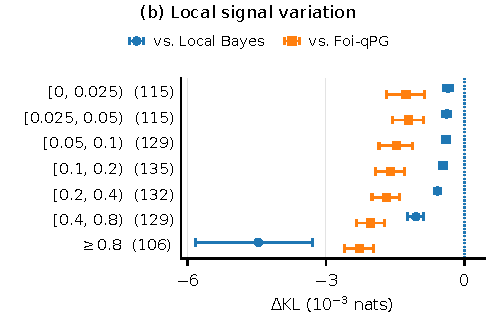
\includegraphics[width=0.493\textwidth]{f10b_holdout_variation.pdf}\\[1pt]
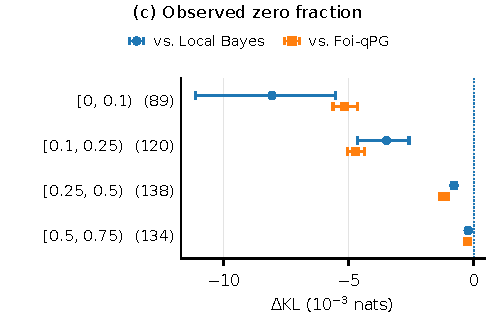
\includegraphics[width=0.493\textwidth]{f10c_holdout_zeros.pdf}\hfill
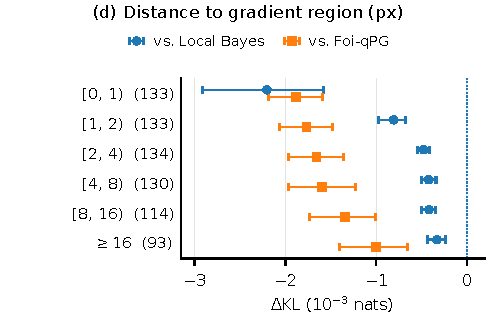
\includegraphics[width=0.493\textwidth]{f10d_holdout_gradient.pdf}
\caption{Regional excess-KL differences on the held-out test set (256-pixel context). Points and 95\% source-bootstrap intervals show N0 minus Local Bayes (circles) or Foi-qPG (squares), where negative values favor N0 and source counts are given in parentheses. Features in (a), (b), and (d) use the simulated signal, whereas the zero fraction in (c) uses the observed RAW input (Supplementary Section~\ref{sec:regionaldefinitions}).}
\label{fig:spatial}
\end{figure*}

\subsection{Role of Spatial Information}
\subsubsection{Cross-CFA Information}
A local estimator can also combine all four CFA phases without a multiscale field. Across 32,462 shared positions from 32 development sources, Joint-CFA Bayes, same-CFA Local PG, and N0 achieve excess KL of 0.001790969, 0.001952344, and 0.000376673~nats, respectively (Supplementary Table~\ref{tab:joint}). While N0 outperforms this local construction, the two estimators also differ in spatial context and prior capacity.

\subsubsection{Location Assignment}
To separate the marginal composition of predicted laws from their spatial placement, we permute the predicted signals across censored positions within each development source and CFA phase, holding calibration parameters and the multiset of predicted laws fixed.

This permutation raises mean excess KL across the 32 sources from 0.0003719 to 0.0026373~nats (assigned minus permuted $-0.0022654$~nats, 95\% interval $[-0.0034895,-0.0012476]$), showing that assigning the same set of distributions to different pixels substantially degrades accuracy.

\subsubsection{Absolute Errors and Signal-Matched Contrasts}\label{sec:gradientcontrol}
Both estimators incur higher error in high-gradient regions, but Local PG rises more steeply. Across the 32 development sources, N0/Local PG excess KL is $0.000191/0.000791$~nats in the low-gradient group and $0.000442/0.002109$~nats in the high-gradient group. The paired KL difference (N0 minus Local PG) shifts by a mean of $-0.001066$~nats from low to high gradient (median $-0.000102$, 23 of 32 sources negative). After matching within source, CFA phase, and signal bins across 27 sources, the mean shift remains $-0.000268$~nats (Supplementary Section~IV).

\subsection{Calibration and Model Mismatch}
N0's 90\% equal-tail integer intervals cover 91.817\% of held-out codes, compared with 91.853\% for the known-signal reference, and Supplementary Table~\ref{tab:coverage} evaluates coverage against exact predicted interval mass across four nominal levels. Under six development stress settings with perturbed read noise or unmodeled row and column offsets, N0 maintains lower mean NLL and CRPS than Local PG (Supplementary Fig.~\ref{fig:pairedstress}).

\subsection{Conditional Distributions of Real Sensor Readouts}
Two 24-megapixel exposures, P2654748 and P2654749, retain signed sensor codes below the nominal black level. Phase-specific integer shifts calibrated from ten dark frames define the hidden reference $V$, while both methods receive only $Y=\max(V,0)$ (Supplementary Section~V). Across six fixed ROIs per exposure, the primary R/$G_1$/$G_2$ sets contain 12,652 and 19,200 censored candidates. The B phase participates in the network input and sampled output, but its real-data scores are diagnostic because its sensor statistics differ. Here local estimators use a $3\times3$ same-CFA window.

\begin{table}[t]
\centering
\caption{Real signed-readout case study on shared R/$G_1$/$G_2$ candidates under the fixed real-data protocol. NLL is in nats per candidate and CRPS is in DN (lower is better).}
\label{tab:real}
\footnotesize
\begin{tabular}{@{}lrrrr@{}}
\toprule
& \multicolumn{2}{c}{P2654748} & \multicolumn{2}{c}{P2654749}\\
\cmidrule(lr){2-3}\cmidrule(l){4-5}
Method & NLL & CRPS & NLL & CRPS\\
\midrule
Global PMF & 3.980276 & 8.289612 & 4.005568 & 8.347404\\
Global PG & 3.979631 & 8.283446 & 4.004966 & 8.341612\\
Local PG & 3.975846 & 8.248081 & 4.004176 & 8.331820\\
Local Bayes & 3.978475 & 8.273926 & 4.006270 & 8.352316\\
Foi-qPG & 3.979516 & 8.283580 & 4.006041 & 8.350880\\
N0/PG & \textbf{3.974503} & \textbf{8.237064} & \textbf{4.003213} & \textbf{8.322619}\\
\bottomrule
\end{tabular}
\end{table}

In P2654748 and P2654749, N0 improves upon Local PG by 0.001342 and 0.000964~nats in NLL and by 0.011017 and 0.009200~DN in CRPS (Table~\ref{tab:real}), with lower NLL in five of six ROIs in the first exposure and two of six in the second (Supplementary Section~\ref{sec:realcode}).

However, the calibrated PG model severely underpredicts the extreme negative tail. Among 31,852 candidates, $V\leq-128$, $V\leq-256$, and $V\leq-305$~DN occur 122, 21, and 13 times empirically, compared with $9.01\times10^{-3}$, $3.76\times10^{-20}$, and $8.63\times10^{-30}$ predicted events. Excluding deep-tail events or repeated coordinates preserves N0's paired NLL advantage over Local PG (Supplementary Table~\ref{tab:real_robust}).

\subsection{Impact on Demosaicking and Shadow Color}\label{sec:downstream}
\subsubsection{Demosaicked Statistics on Real Exposures}
We demosaic the retained signed reference, clipped version, N0 samples, and Local PG samples with the same LibRaw AHD implementation, adding a 512-DN digital pedestal for unsigned LibRaw processing and subtracting it in linear camera RGB prior to color rendering.

Across 32 separately demosaicked draws in the darkest ROI of P2654748, clipping raises the linear G mean from 9.003 to 16.322~DN, which N0 and Local PG restore to 8.621 and 8.602~DN, while clipping reduces the spatial standard deviation of $R-G$ from 25.986 to 18.635~DN, which N0 and Local PG restore to 25.157 and 25.256~DN. Conditional sampling thus recovers most of the shadow variation removed by censoring, with similar statistics from both estimators (Supplementary Table~\ref{tab:ahd}, Supplementary Section~V, and \href{visual_en.pdf}{Supplementary Visual A}).

\subsubsection{Clean-Reference Shadow Color in Synthetic Scenes}
A development experiment evaluates rendered shadow color across eight natural scenes and four procedural templates after AHD, fourfold signed-domain averaging, and fixed white balance, color conversion, and exposure scaling, measuring squared block-mean $(R-G,B-G)$ error in exposure-scaled linear display RGB against the demosaicked quantized clean signal $Q(s)$ (Supplementary Section~\ref{sec:cleanendpoint}).

Across the eight natural scenes, direct clipping raises color error from 0.125006 (signed readout) to 1.257683 (Table~\ref{tab:cleanendpoint}). Conditional sampling reduces this error to 0.122891 for N0 and 0.126031 for Local PG, a paired N0-minus-Local difference of $-0.00314$ (95\% source-bootstrap interval $[-0.00614,-0.00084]$, or 2.49\%). Quantized conditional means (\emph{mean-$Q$}) yield 0.102618 and 0.105440.

\begin{table}[t]
\centering
\caption{Shadow-color error and clean-RAW MSE across eight natural development sources (equal source weights). Color error is squared block-mean $(R-G,B-G)$ error in exposure-scaled linear display RGB, and RAW MSE is relative to $Q(s)$ in DN$^2$. The original signed row uses the uncensored noisy readout (lower is better for both).}
\label{tab:cleanendpoint}
\small
\setlength{\tabcolsep}{4pt}
\begin{tabular}{@{}lrr@{}}
\toprule
RAW input & Dark-color error & RAW MSE\\
\midrule
Original signed & 0.125006 & 1157.747\\
Directly clipped & 1.257683 & \textbf{866.698}\\
Local PG sampled & 0.126031 & 1157.244\\
N0/PG sampled & \textbf{0.122891} & 1159.305\\
Local PG mean-$Q$ & 0.105440 & 1077.675\\
N0/PG mean-$Q$ & \textbf{0.102618} & 1076.179\\
\bottomrule
\end{tabular}
\end{table}

For any nonnegative clean reference $c=Q(s)$ and any allowed fill $k\leq0$, $(k-c)^2-c^2=k^2-2kc\geq0$. Zero fill ($k=0$) therefore minimizes pixelwise clean-RAW MSE among measurement-preserving methods, yet by shifting shadow means it produces the largest block color error in Table~\ref{tab:cleanendpoint}, whereas quantized conditional means achieve the lowest color error.

\subsection{Runtime and Full-Resolution Inference}\label{sec:runtime}
On an RTX 3090~Ti, completing a 24-megapixel frame takes 27.3901~s with N0/PG and 205.1503~s with Local PG, with peak allocated CUDA memory of 750.69 and 94.84~MiB (Supplementary Table~\ref{tab:runtime}). Full-resolution inference uses phase-aligned overlapping tiles (Supplementary Section~VI), and coordinate-indexed sampling is invariant to tile order for fixed laws (Supplementary Section~III).

\section{Discussion}
The held-out experiments link conditional readout accuracy directly to where predicted distributions are placed in space. Where the signal varies across edges and textures, locally constant models incur larger errors and multiscale estimation provides clear gains. Permuting the locations of N0's predictions while keeping their collection fixed increases excess KL, confirming that spatial assignment is a primary source of completion accuracy.

While distribution scores measure the accuracy of the conditional readout law itself, downstream statistics also depend on demosaicking and color processing. Synthetic experiments under matched PG physics use the known-signal law to isolate estimation error. On real exposures, the shared Gaussian noise model severely underpredicts rare deep-negative codes, yet N0 retains a consistent paired likelihood advantage. Both samplers recover demosaicked shadow variation, and our controlled rendering test shows that although zero fill minimizes clean-RAW MSE, restoring below-zero readouts prevents shadow color bias.

\section{Conclusion}
A single zero in a lower-censored RAW image can correspond to multiple signed integer readouts. N0/PG estimates each pixel's discrete conditional law from surrounding Bayer measurements, sampling only at censored positions while preserving all positive codes. Across 138 held-out sources, this spatial estimator consistently outperforms global, local-likelihood, and transform-domain baselines, while real signed readouts and fixed-rendering experiments demonstrate how missing negative codes preserve shadow statistics and color.

\section*{Reproducibility Statement}
The accompanying repository provides table scores, source identifiers, color evaluation records, trained weights, and inference and evaluation code, verified in an isolated environment with SHA-256 manifests. Original code and weights use the MIT License, original figures and numerical results use CC BY 4.0, and third-party materials retain their respective licenses.

\bibliographystyle{IEEEtran}
\bibliography{references}
\end{document}
